% 2011 年重庆卷文科第 20 题：四面体 ABCD，平面 ABC⊥平面 ACD。
% 来源 PDF：普通高考/2011/2011重庆文.pdf，SHA-256 0ddbe738e4414213612fb6f62ec0c5cd252d039abf560bae1f31610558f93a70。
% 原页：第 2 页第 2 栏上部，书页码 654。示意。
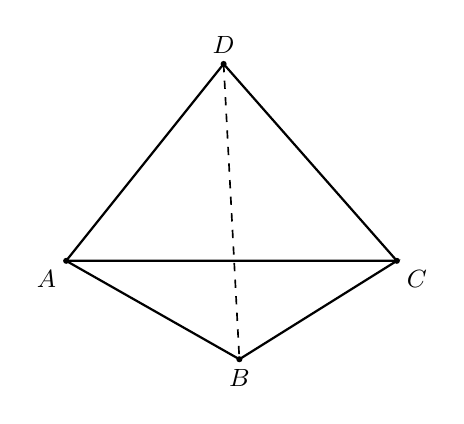
\begin{tikzpicture}[>=stealth, semithick, font=\small, scale=1.0]
  \coordinate (A) at (0,0);
  \coordinate (C) at (4.2,0);
  \coordinate (B) at (2.2,-1.25);
  \coordinate (D) at (2.0,2.5);
  \draw[thick] (A)--(B)--(C)--(A);
  \draw[thick] (D)--(A) (D)--(C);
  \draw[dashed] (D)--(B);
  \fill (A) circle (1.1pt) node[below left] {$A$};
  \fill (B) circle (1.1pt) node[below] {$B$};
  \fill (C) circle (1.1pt) node[below right] {$C$};
  \fill (D) circle (1.1pt) node[above] {$D$};
\end{tikzpicture}
